\section{Introduction}
Machine learning is becoming increasingly pivotal in a variety of critical
applications. Its usage extends to healthcare tasks such as detecting cancer
\citep*{breast_cancer_prognosis} and predicting diabetes outbreaks
\citep*{diabetes_classification}, underscoring its importance in public health and safety. 
Additionally, machine learning plays a significant role in environmental sustainability,
for example in forecasting energy usage \citep*{energy_forecasting},
which is essential for efficient resource management. Beyond these critical
areas, it also enhances everyday technology experiences, like search engine page 
rankings \citep*{page_ranking}, demonstrating its broad impact across diverse aspects of daily life.

Therefore it is essential to be able to train accurate and robust models. With
Ensemble Learning methods such as Bagging \citep*{Breiman1996},
Boosting \citep*{Schapire1990}, Random Forest \citep*{breiman2001random},
and Gradient Boosting \citep*{breiman1997arcing, friedman2001greedy, friedman2002stochastic}
it is possible to reduce the bias, variance and to create more resilient, robust,
and generalized models. Thereby improving the overall accuracy and outperforming
individual learning algorithms.
Furthermore, Ensemble Learning methods are able to manage complex datasets
characterized by noise, imbalance, and high dimensionality, as well as effectively
hanlding missing data.

As a part of the proseminar "Advanced topics in machine learning", this report
aims to provide a comprehensive overview of Bagging, Boosting, and Ensemble 
Learning, explaining how they work, why they are important in the field of 
machine learning, and comparing them on real world datasets.

% ---------------------------------------------------------------------------- %
\section{Ensemble Learning}

Ensemble learning is an advanced machine learning approach that combines the 
strengths of multiple smaller learning algorithms to improve predictive 
performance. 
The concept behind ensemble learning is analogous to the "wisdom of crowds".
Which describes, that a crowd, on average, makes collectively better decisions,
than any single member of it.

Just as a diverse group of people can provide a more accurate collective decision 
than an individual, in ensemble learning, a combination of learning algorithms
often predicts more accurately than an individual learning algorithm.
This approach is based on the principle that a diverse set of learning algorithms
can capture different patterns or trends in the data, leading to more robust and 
accurate predictions.

To be more precise, ensemble methods use multiple smaller learning algorithms,
which specialize in small aspects of the problem. However, by combining these
algorithms, the ensemble often achieves better predictive performance than 
the used algorithm could achieve alone because they complement each others
strengths and weaknesses.

So the goal of ensemble learning is to achieve a better predictive performance.
Nevertheless, it comes at the cost of increased computational resources for 
training as well as prediction and storage.

Overall, there are many different ensemble methods, such as Bagging and Boosting, 
which we will go into more detail in this report.
% ---------------------------------------------------------------------------- %
\subsection{Bagging}

% Intro Bagging and Traing
Bootstrap Aggregating, commonly known as Bagging, is an ensemble learning method
developed by \citet*{Breiman1996}. The models for the ensemble get trained individually
by using the bootstrapping technique. Bootstrapping involves creating random
subsets of the original training dataset. The subsets are created by drawing 
random data points with replacement and have the same size as the original
training dataset. This means that data points can be chosen more than once and
that some data points might not be in the subset. The models can be trained in
parallel, because of the individually created subsets.


\hyperref[fig:bootstrapping]{Figure 1} shows how bootstrapping might work on an imaginary dataset. In subset 1
each class is equally distributed. Subset 2 has a focus on the red and orange bubbles.
The subset N has a strong focus on blue, however it doesn't even have a single 
orange bubble. This will probably mean that the model trained on subset N will be very
good at predicting blue, but not very accurate with orange.

\begin{figure}[htbp]
    \label{fig:bootstrapping}
    \centering
    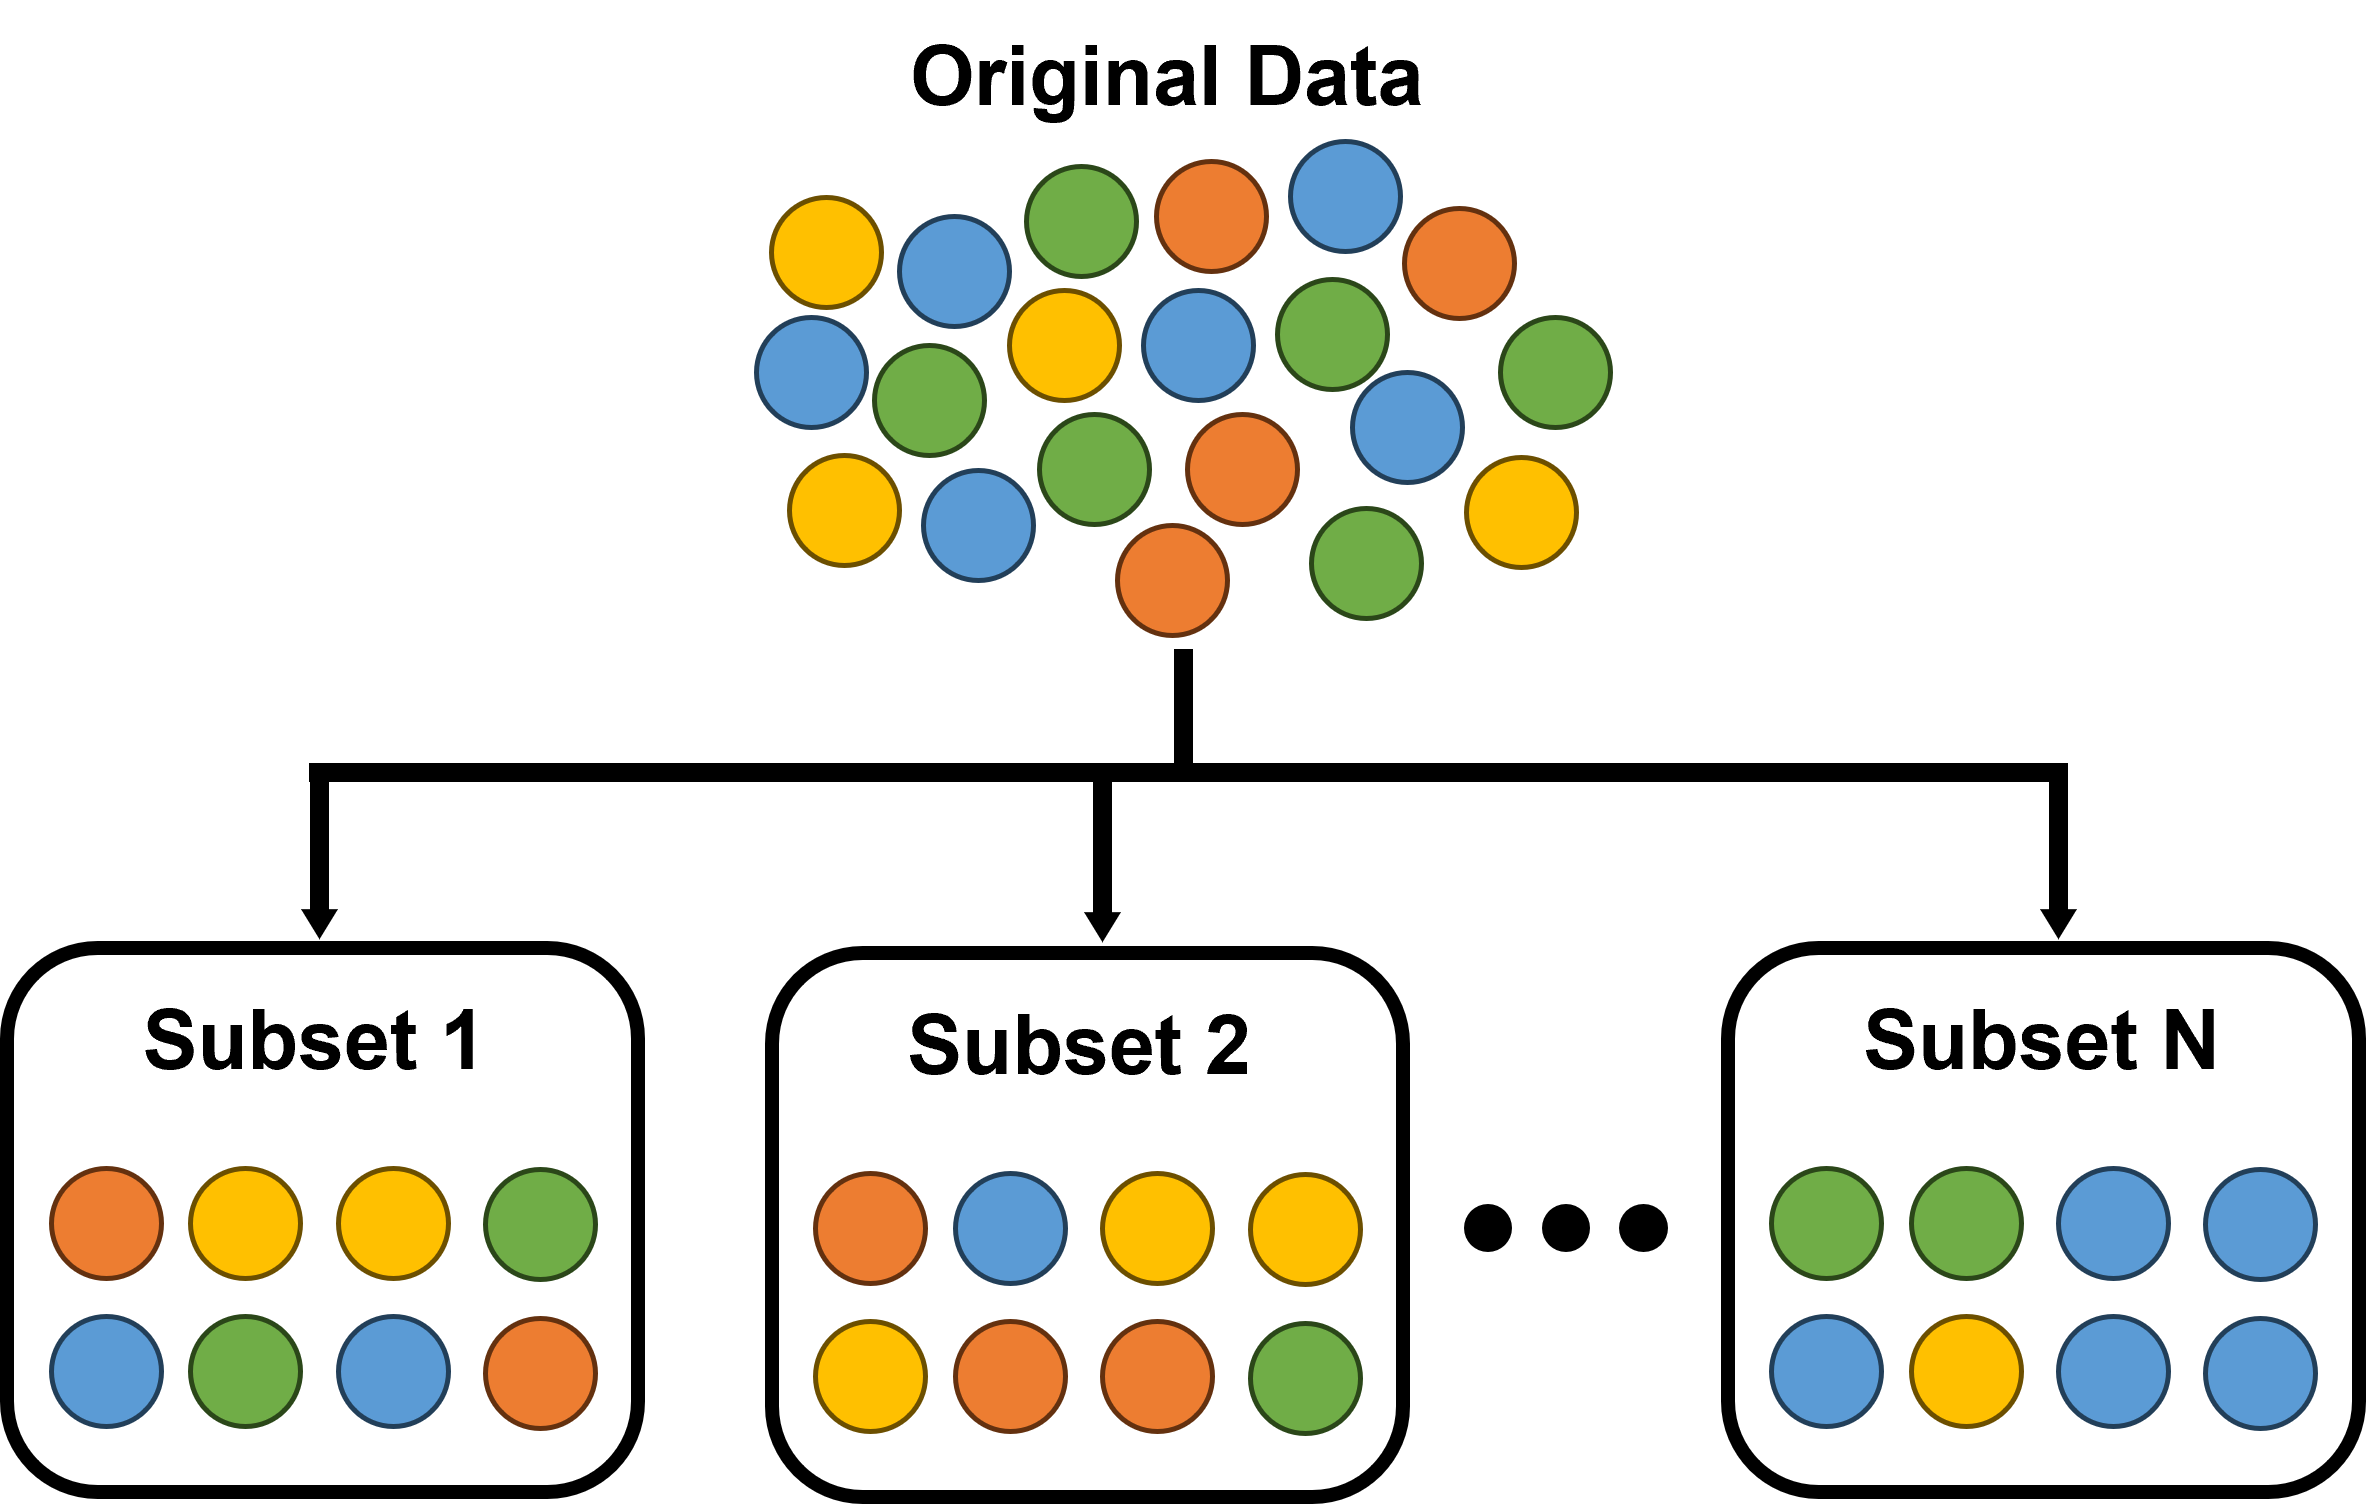
\includegraphics[width=.6\textwidth]{figures/bootstrapping}
    \caption{Creating subsets with bootstrapping.}
\end{figure}

% Prediction Bagging
In the Bagging ensemble, each model makes its prediction independently. Because of
that the predictions of the individual models can be run in parallel, similar to
the training. Once every model in the ensemble has made their prediction, they get
aggregated to form a final ensemble prediction. The method of aggregation depends
on the problem that is being solved by the Bagging ensemble. 
For classification problems, a common method is majority voting. Each model votes 
for a particular class. The class that receives the most votes is chosen for the
final ensemble prediction.
For regression problems, the predictions of the individual models are typically 
averaged.

\begin{figure}[htbp]
    \centering
    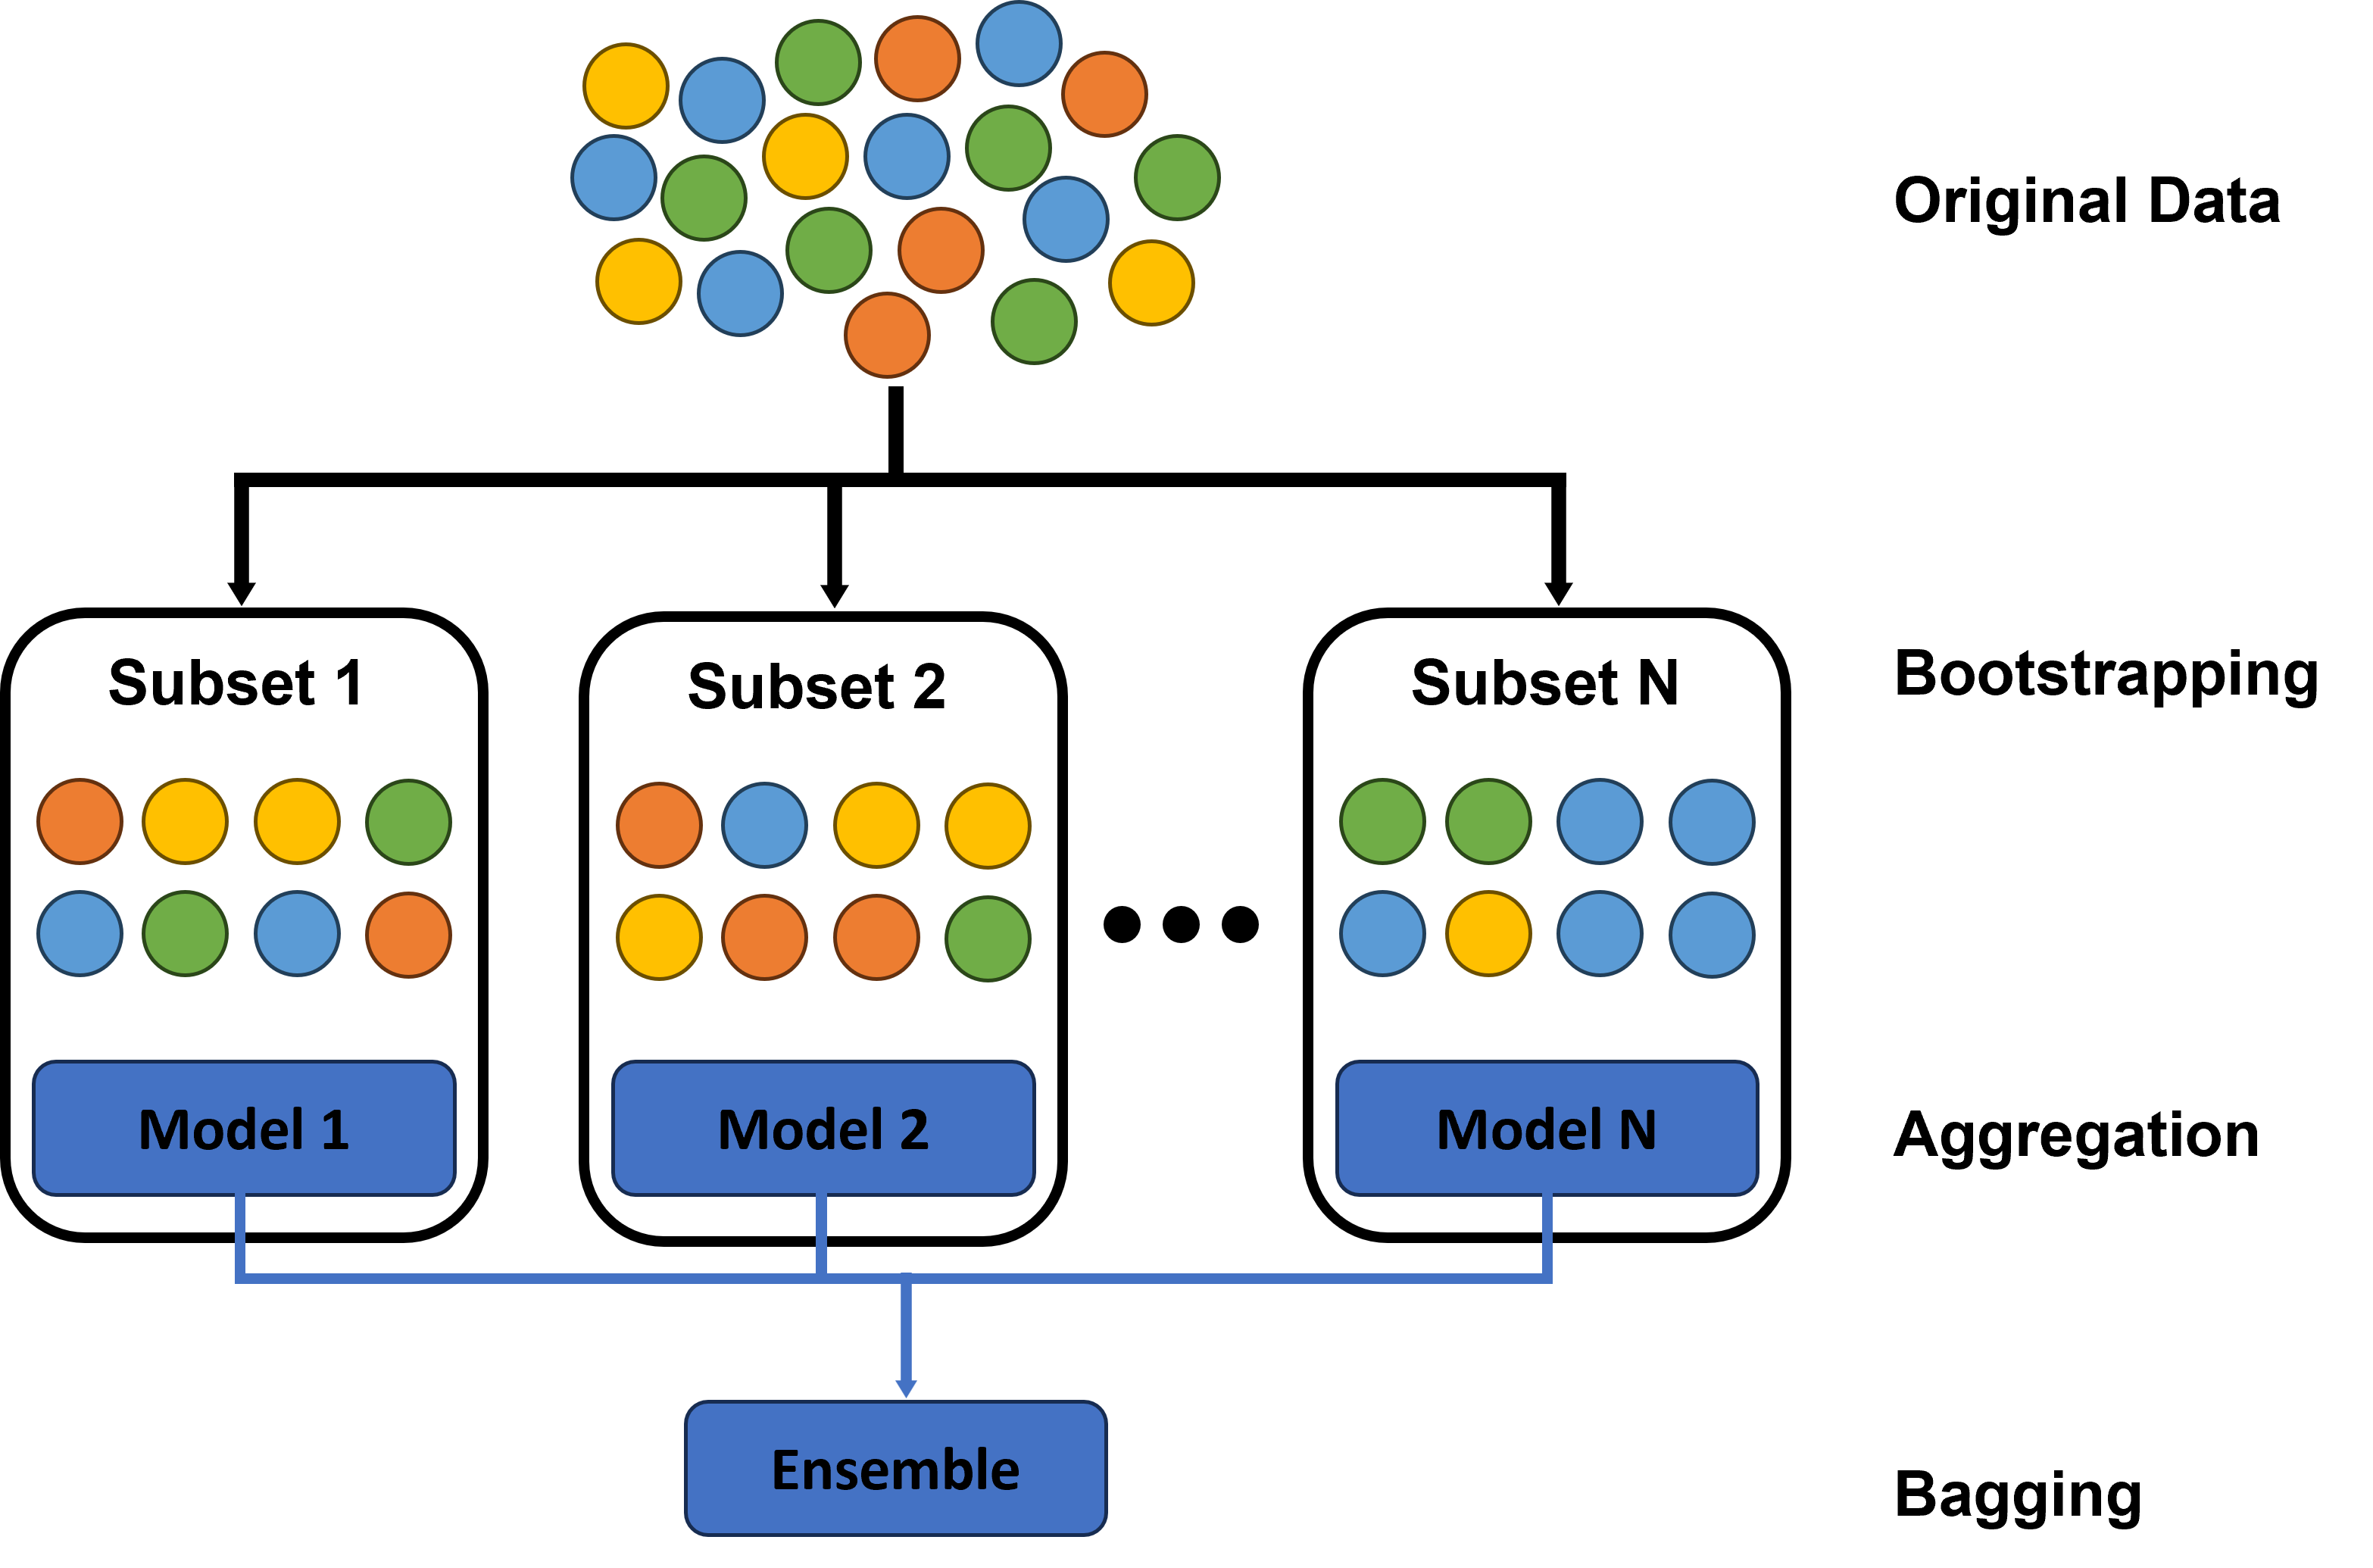
\includegraphics[width=.65\textwidth]{figures/bagging_prediction}
    \caption{Bagging prediction example}
\end{figure}

\newpage
% When to use bagging (Advantages)
% Utilizing Multiple Cores for Parallel Training / Prediction could be added
Bagging can be particularly effective when using base learning algorithms
that have high variance or tend to overfit quickly. By bootstrapping and 
averaging the predictions, the variance gets reduced and potential overfitting
is avoided.
The same goes for unstable learning algorithms, that produce significantly different
results on small changes in the data. That's why Bagging is often used with Decision
Trees as they tend to be unstable and to have high variance.
Additionally, Bagging can be very helpful when dealing with noisy, imbalanced 
datasets or datasets with missing data. The bootstrapping helps to create 
diverse datasets with each class being adequately represented and also averaging
out the noise in combination with aggregation.


% Summary
All in all, Bagging can help to reduce variance, prevent overfitting, and to build
a more resilient, robust, and generalized model.

\subsection{Random Forest}
Random Forest is an ensemble learning method, like Bagging, also developed
by \citet{breiman2001random}. The difference between Bagging and Random Forests
lies in the training of the models within the ensemble. 
First, the base learning algorithm is always a Decision Tree. 
Second, Random Forests utilize a method called feature randomness. When building
each tree within a Random Forest, a random subset of features is chosen for consideration
at each node, rather than using all available features for the splits.
Because of that, Random Forest typically requires to use more models within the ensemble
than Bagging.
This randomness reduces the correlation between the individual trees, avoiding
overfitting and increasing robustness and generalization. This often results in
Random Forests being more accurate than Bagging.

\subsection{Out-of-bag}

Out-of-bag (OOB) by \citet{breiman1996out} is an useful concept for Bagging and Random Forest. 
It provides a way to measure the performance of the model without needing a separate validation set. 
Because of the way Bagging and Random Forest are trained, the Decision Trees are on average
only trained on around 63\% of the data, and they don't see around 37\%. 
Therefore we can evaluate the ensemble on the training set. For each data point, we only use
the Decision Trees that did not see the examples during the training step. By averaging the
performance of that step, we receive an out-of-bag error.
The OOB error can then be used to tune the hyperparameters of the model. Out-of-bag is particularly
useful for small datasets, as it allows the use of the entire dataset for training while still
providing an unbiased estimate of model performance.
While OOB error is a useful tool for model assessment, it may not always perfectly align with the
error estimated on an independent validation set.

\hyperref[fig:oob]{Figure 3} shows how out-of-bag might work on an imaginary dataset.
The first subset doesn't contain the data points 2, 5, and 6. Therfore the Decision
Tree that is trained on the first subset will be able to use those data points for testing.
This works exactly the same for all other subsets.

\begin{figure}[htbp]
    \label{fig:oob}
    \centering
    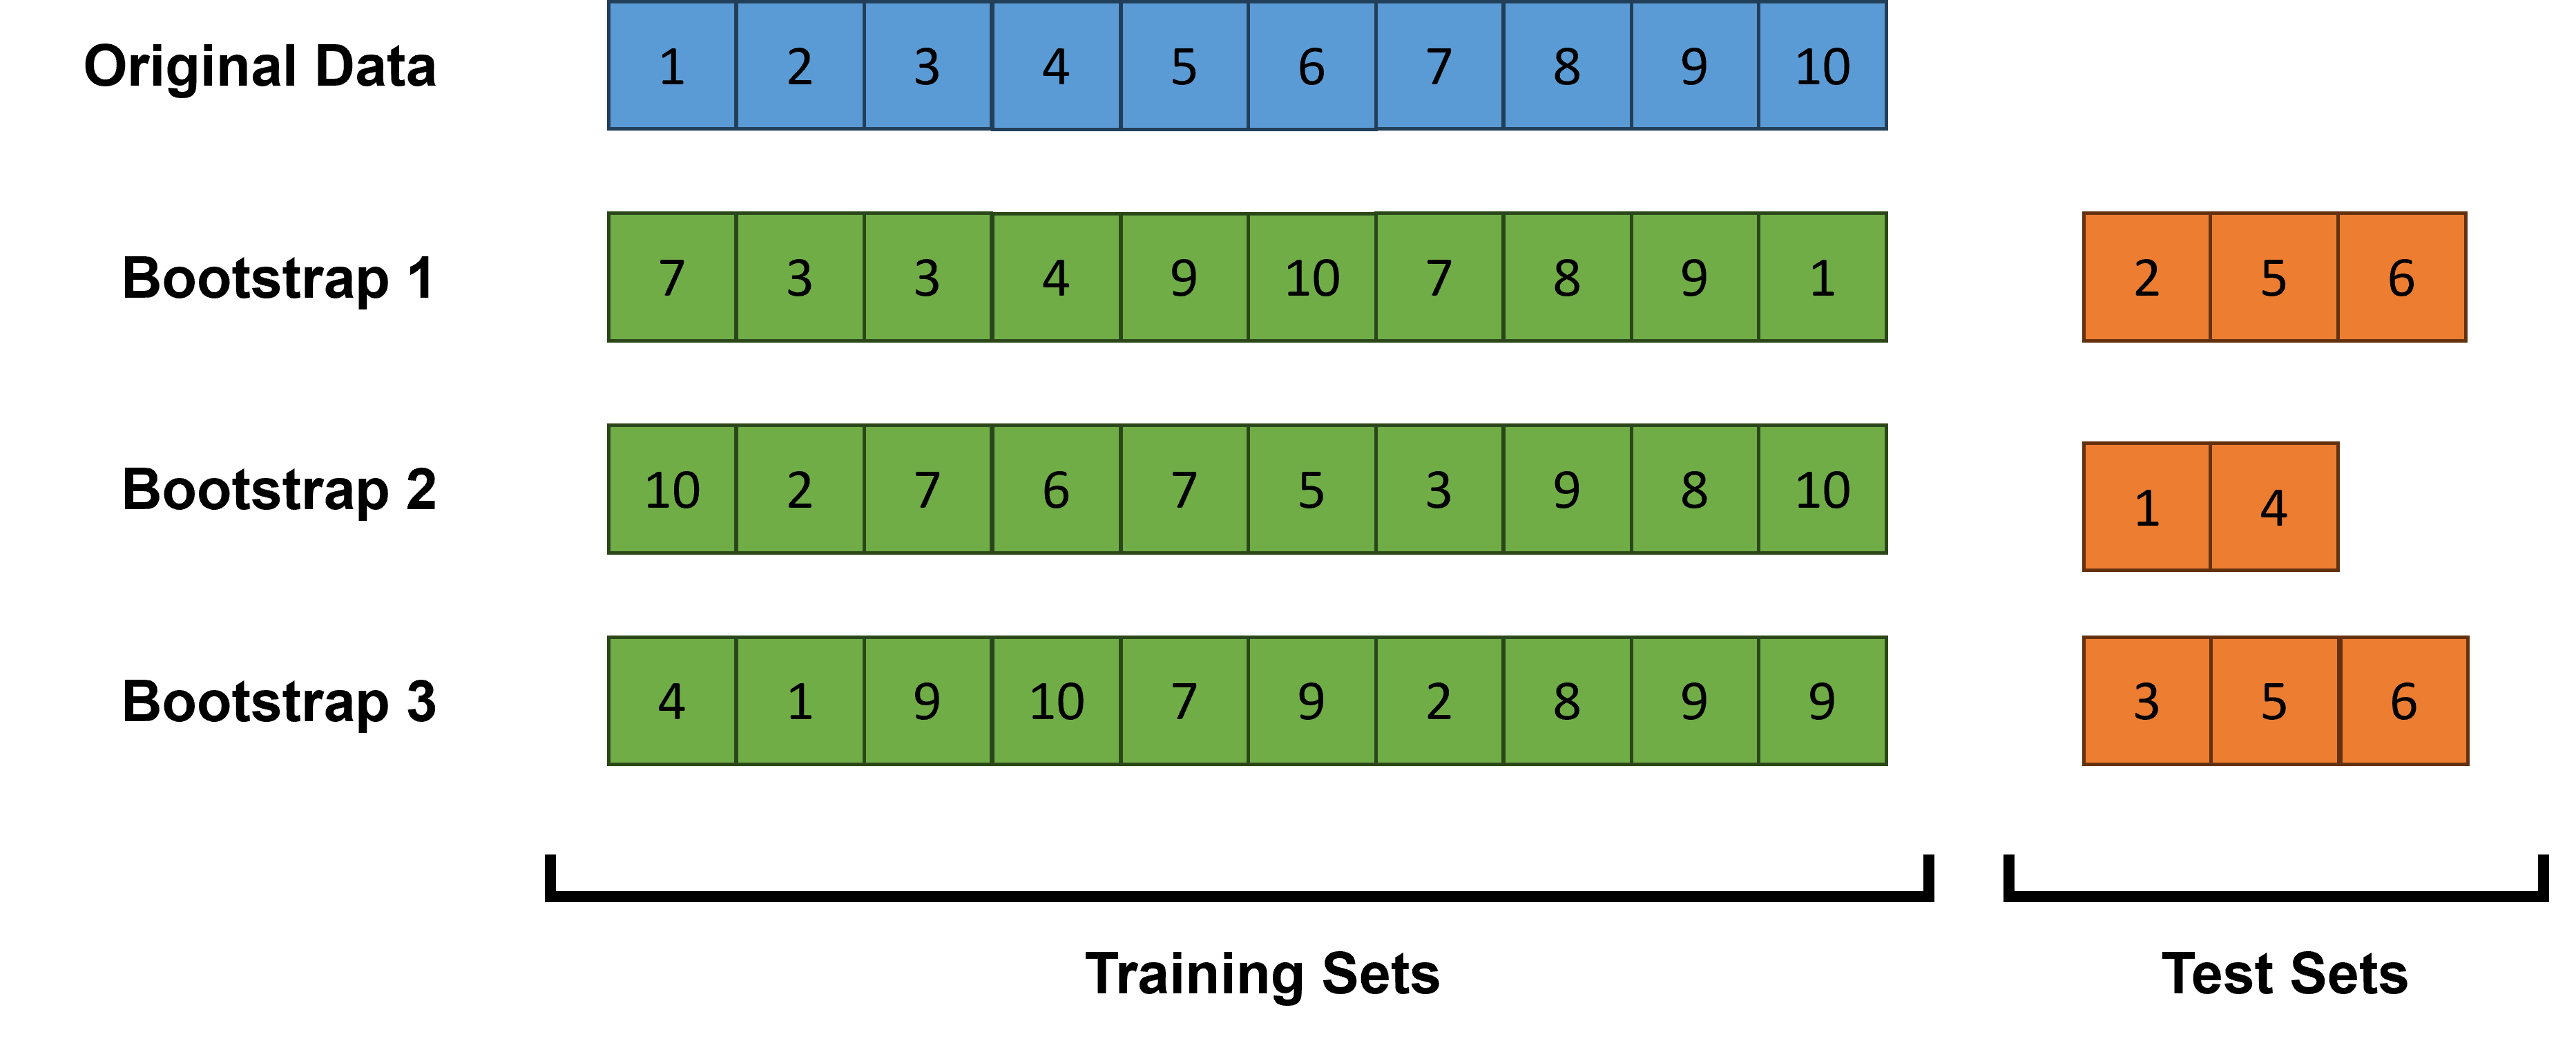
\includegraphics[width=.8\textwidth]{figures/out_of_bag}
    \caption{Out-of-bag example}
\end{figure}

% ---------------------------------------------------------------------------- %
\subsection{Boosting}
Boosting \citep{Schapire1990} is another ensemble learning method like Bagging.
However, unlike Bagging, Boosting trains the models sequentially, where each
model learns from the mistakes of its predecessors.
In the first step, the data subset for the first model gets created and a model 
is trained on it. Initially, the dataset is equally weighted, similar to the initial
setup in Bagging: data points are drawn with replacement until the subset has the 
same size as the original dataset.
In the second step, the performance of the model is evaluated. The weight gets
increased for incorrectly predicted samples and decreased for correctly predicted
samples. 
In the third step, the next model is trained on the dataset with the updated weights.
This weight adjustment makes the next model focus more on the data points that 
previous models predicted incorrectly.
Steps two and three, the process of updating weights and training new models now gets 
repeated until all models are trained.
Different from Bagging, Boosting can't be trained in parallel, because each model
is trained based on the previous model's performance. 

\begin{figure}[htbp]
    \centering
    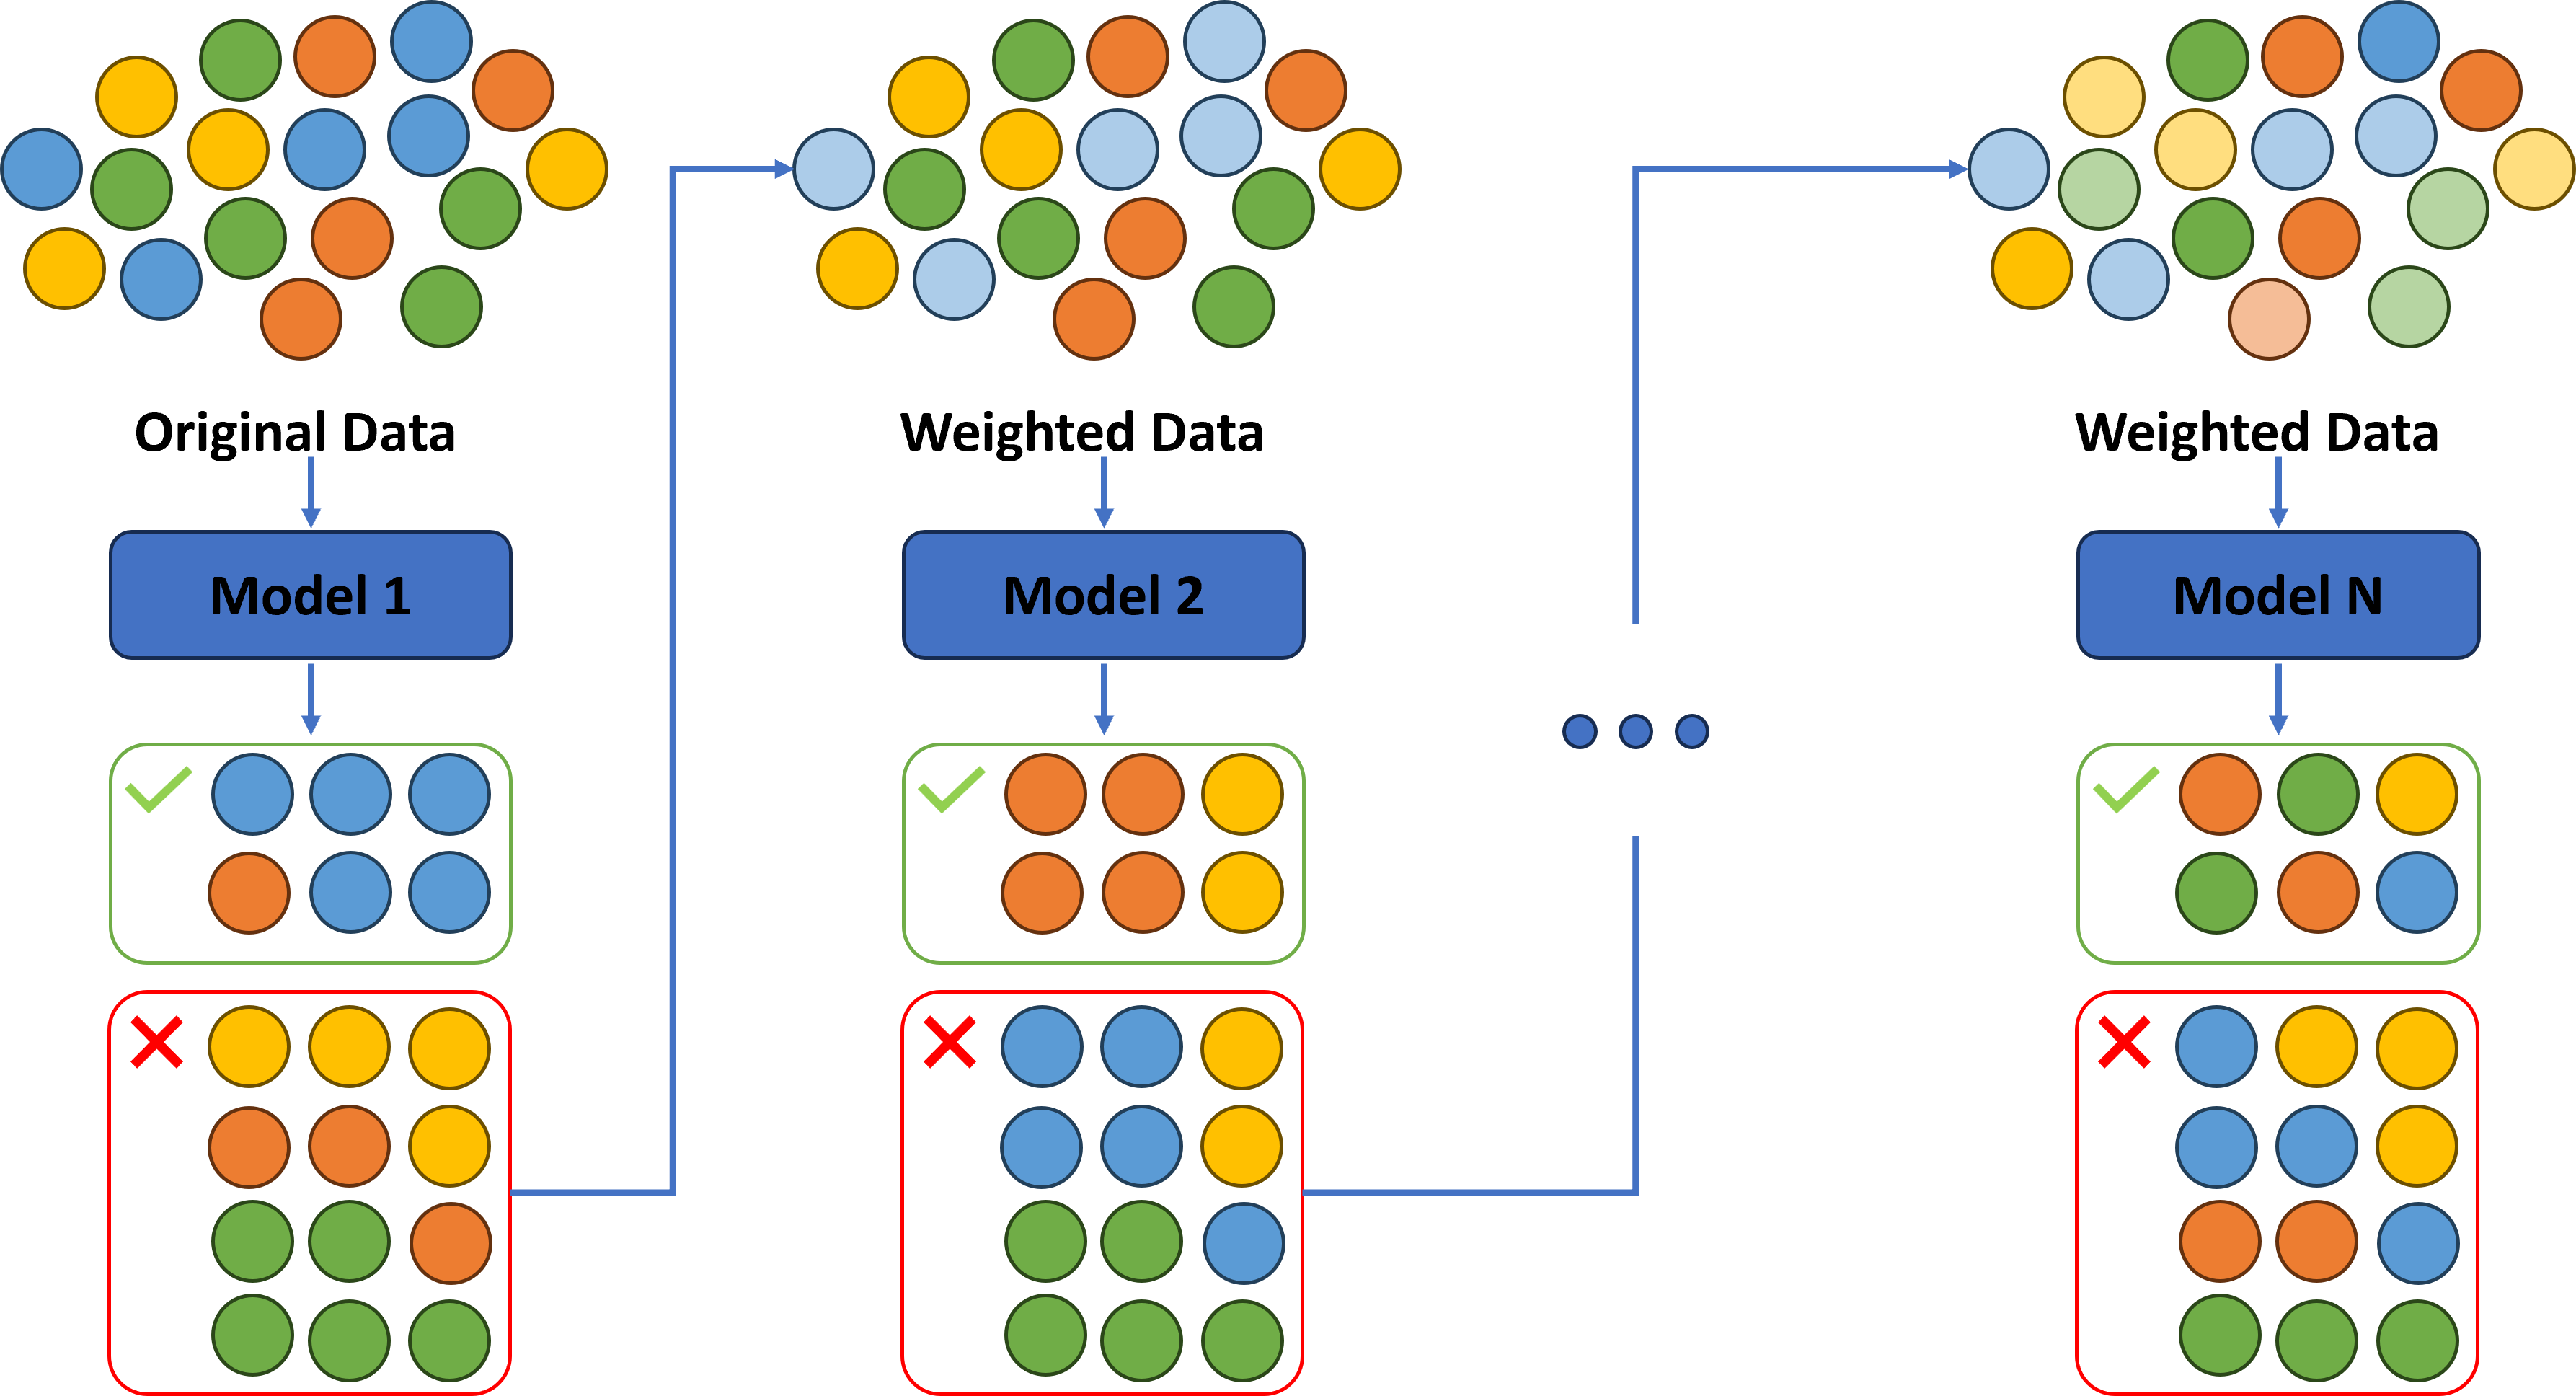
\includegraphics[width=.7\textwidth]{figures/boosting_training}
    \caption{Boosting training example}
\end{figure}

% Boosting prediction
In contrast to the training, each model makes its individual prediction in Boosting.
This means the predictions can be done in parallel.
Unlike Bagging where each model's prediction is given equal weight, Boosting uses
a weighted average approach to combine the individual predictions. This means
each model has its own weight based on the performance in the training phase.
For classification problems, this means that the vote of each model can have
a different influence on the final ensemble prediction.
In the case of regression problems, the final prediction is the weighted average
of the predictions from all models.

% When to use boosting (Advantages)
Boosting is ideal to use when the base learning algorithm suffers from high bias.
This is combated through the way the ensemble is trained, as each model focuses on the
weaknesses of the previous one.
Additionally, Boosting is particularly effective with high-dimensional data, where
the number of features is large. Other models might not be able to capture the 
complexity or more complex models might overfit.
However, Boosting can strike a balance by incrementally building complexity and 
focusing on features that improve the predictive performance.
Furthermore, it's important to note that Boosting works best on datasets with little 
to no outliers. The ensemble strongly focuses on correcting errors. Outliers can 
disproportionately influence the direction of the learning process, leading
to overfitting.


% Boosting summary
To put it in a nutshell, Boosting can help to reduce bias, avoid underfitting,
and can help to build overall precise models. Nevertheless, you have to be aware
of the challenges with Boosting e.g. noisy data.

\subsection{Gradient Boosting}
Gradient Boosting \citep{breiman1997arcing, friedman2001greedy, friedman2002stochastic} 
is an ensemble learning method similar to Boosting. It is typically, but not solely used in 
combination with Decision Trees. Also called Gradient-Boosted Trees.

For regression tasks, Gradient Boosting starts with making a naive prediction on the target,
by using the mean of the target derived from the training data as the inital prediciton.
To achieve better accuracy, the Gradient Boosting algorithm places its focus on the
residuals (difference between target and predicted value). The primary objective is to minimize
them systematically.
In order to do that, it builds a Decision Tree, that tries to predict the calculated residuals.
Unlike regular Boosting, Gradient Boosting is using deeper Decision Trees with usually around 8 to 32 leafes.
Now new predictions are made by using the Decision Tree to predict the residulas, multiply them
with a learning rate, and adding them to the calculated mean.
With the new predictions, the residuals are recalculate and the next Decision Tree is fit on to them. 
This process gets repeated until a predetermined number of Decision Trees are added to the ensemble
or when the models improvements fall under a given threshhold.

\begin{figure}[htbp]
    \centering
    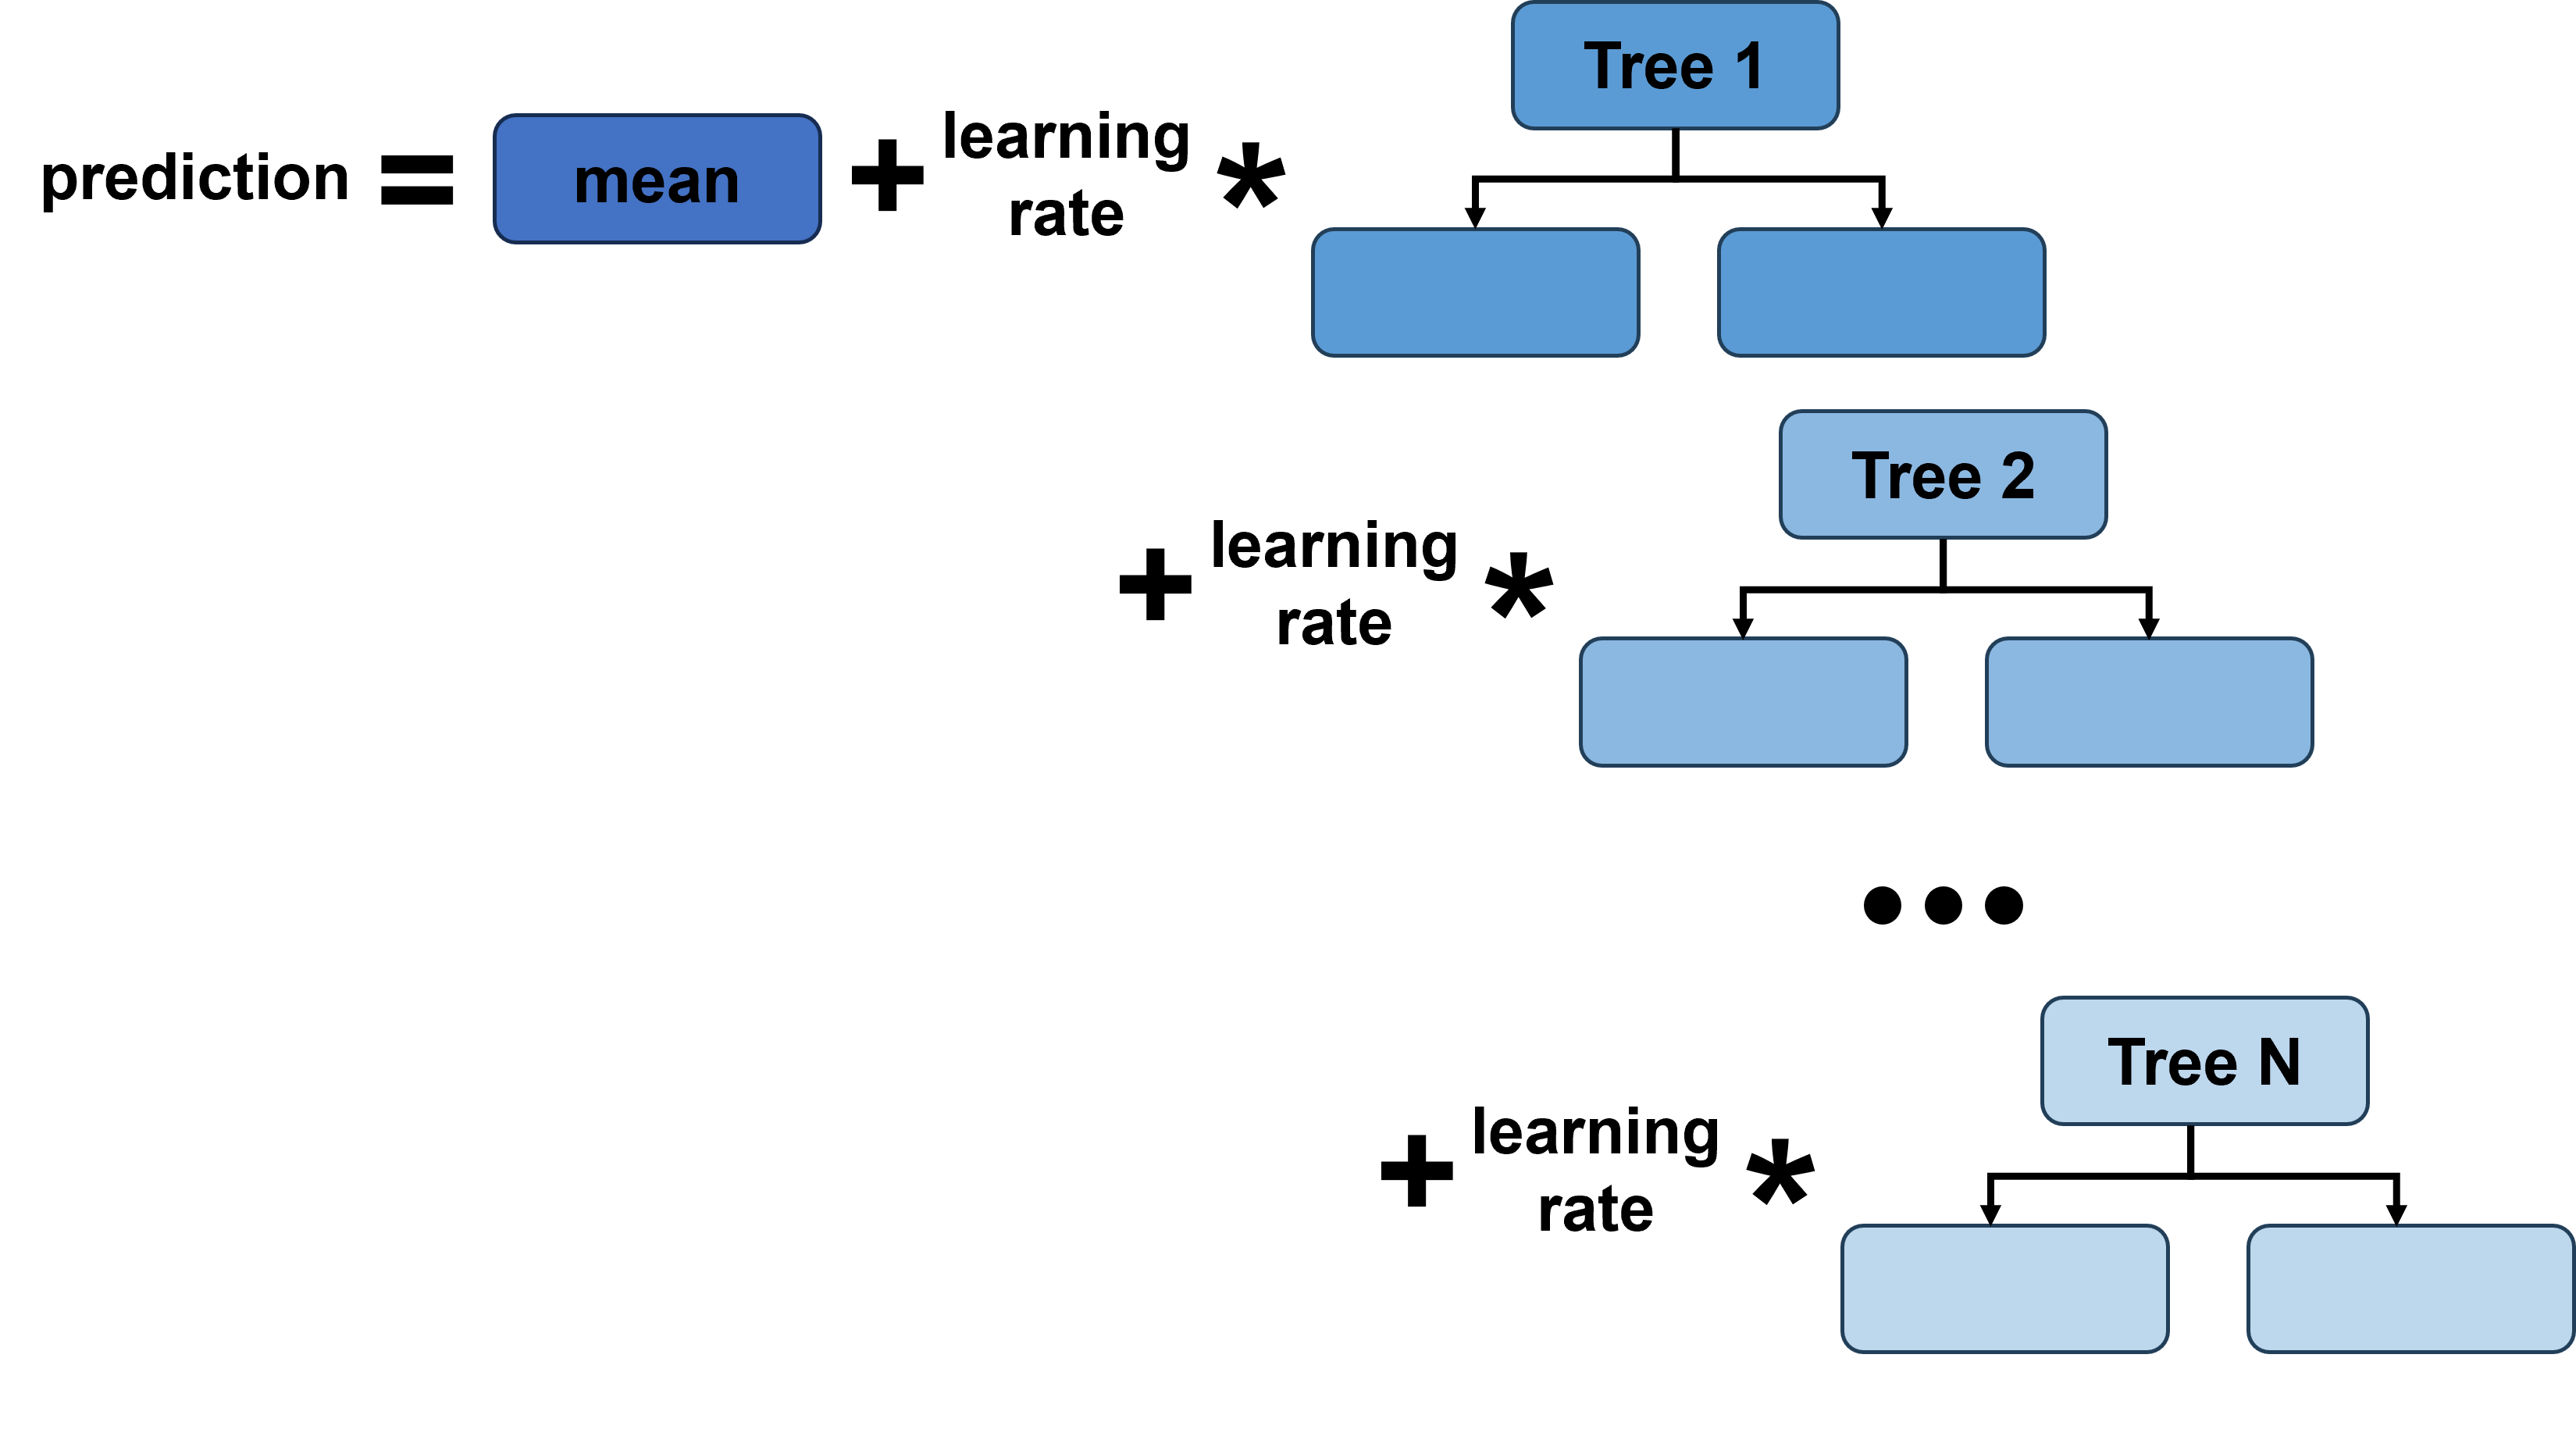
\includegraphics[width=.8\textwidth]{figures/gradient_boosting_prediction}
    \caption{Gradient Boosting regression prediction example}
\end{figure}

For classification tasks, similar to regression, a naive prediction is being calculated.
The way this is done depends on the implementation of Gradient Boosting. It can be the proportion of one
class or it could be the log of the odds (logit) converted into a probability by putting it into sigmoid.
Then the residuals are calculated by substracting the naive prediction from the class, and fits a Dicision
Tree on them with in order to minimize the residuals.
However in difference to regression, the Decision Tree values and the naive prediction can't just be added
together. Thats because the naive prediction is in terms of the logit, and the result from the Deicision Tree is
derived from a probability. Therfore the Decision Tree values must be transformed. The most common formular for
transformation is:

$$\frac{\sum Residual_i}{\sum [Previous \, Probability_i \cdot (1 - Previous \, Probability_i)]}$$

Now the predicitons can be calculated by multiplying the learning rate to the new Decision Tree values and
adding that to the naive prediction. This can then be converted to a probability with sigmoid.
Like before, the new predictions can be used to recalculate the residuals and the next Decision Tree is fit on to them.
The process gets repeated until it hits a stopping criteria. Those can be the same as the ones for regression.

% ---------------------------------------------------------------------------- %
\section{Examples}
In the examples, we aim to compare various ensemble learning algorithms - Bagging, 
Boosting (AdaBoost - \citet{freund1996experiments}), Random Forest, and Gradient 
Boosting - against Decision Trees across different datasets.
First, we are looking for the optimal depth of the Decision Tree which maximizes the 
precision. This Decision Tree will be used as the base learning algorithm for 
the ensemble learning algorithms.
In order to determine the best maximum depth of the Decision Tree, the datasets are 
split into a validation set (20\%) and a training set (80\%). The training set is used
for a 10-fold cross-validation, where the overall accuracy is calculated by averaging the 
accuracy of all folds. With the 10-fold cross-validation of the training set, we are
searching for the best maxmimum depth, trying all of them from 1 to 30. We stopped at
30 as the accuracy declined or stagnated for all examples. The Decision tree with the
best accuracy is then used as the base learning algorithm for the ensembles.

The same method is used to find the best estimator count for Bagging, Boosting, 
Random Forest and Gradient Boosting. However, in contrast to the Decision tree,
we are trying all estimator counts from 1 to 500.
The learning rate is always 0.1 if applicable. Afterwards, the Decision Tree and
the ensemble learning algorithms are tested on the validation set.
This approach allows us to comprehensively assess each algorithm's effectiveness
and draw meaningful comparisons.

The experiments were implemented in Python 3.10.1, using scikit-learn 1.3.2, and
conducted on a system equipped with an AMD Ryzen 5 5600X CPU (3.7 GHz, 6 cores).
The examples are avaialble as an open sources repository on github\footnote[1]{https://github.com/FlorianREGAZ/Bagging-Boosting-Ensemble-Learning}.

\newpage % TODO: remove
\subsection{Example 1}
\label{sec:example1}

In the first example we are using the Breast Cancer Wisconsin (Diagnostic)
dataset by \citet*{breast_cancer_wisconsin}. The dataset originates from
the University of Wisconsin Hospitals. It contains 30 features and has 569
data points. The goal of the dataset is to classify if breast cancer
is benign or malignant (classification).

\begin{table}[htbp]
    \centering
    \begin{tabular}{l c c c c}
    \toprule
    Learning algorithm  & Worst fold     & Best fold     & Average fold  & Validation    \\
    \midrule
    Decision Tree       &  0.85          & 0.98          & 0.93          & 0.93          \\
    Bagging             &  0.84          & \textbf{1.00} & 0.93          & 0.96          \\
    Random Forest       &  0.85          & \textbf{1.00} & \textbf{0.95} & 0.97          \\
    Boosting            &  0.87          & \textbf{1.00} & \textbf{0.95} & \textbf{0.99} \\
    Gradient Boosting   &  \textbf{0.89} & \textbf{1.00} & 0.94          & \textbf{0.99} \\
    \bottomrule
    \end{tabular}
    \caption{Breast Cancer Wisconsin (Diagnostic) model accuracy}
\end{table}

\begin{figure}[htbp]
    \centering
    \label{fig:bcw_comparison}
    \makebox[\textwidth]{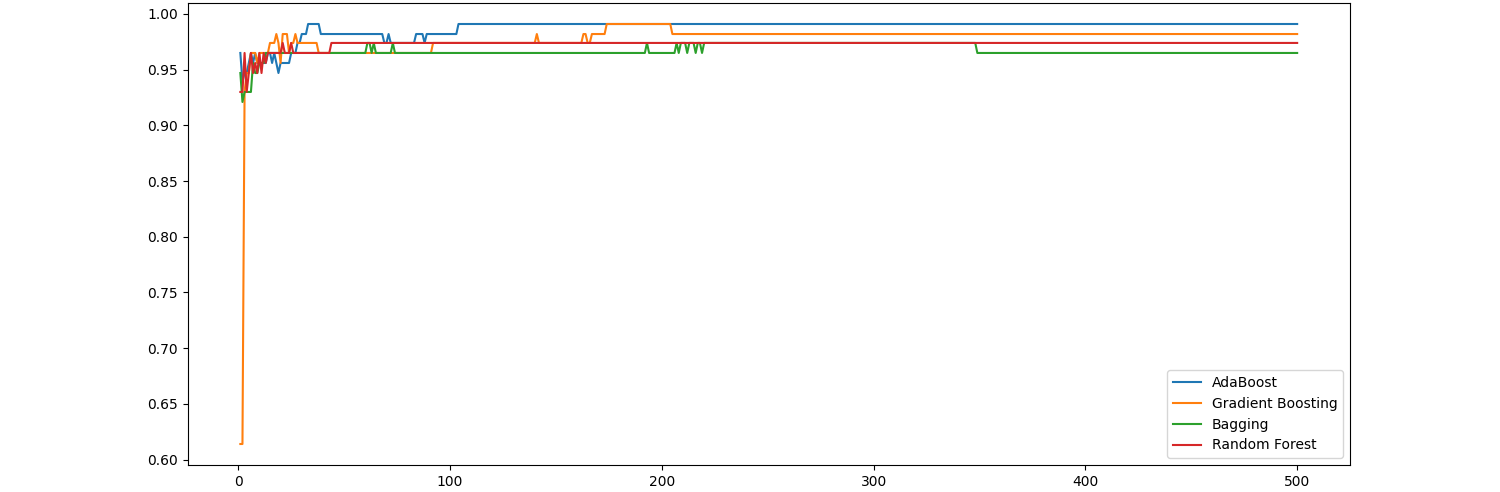
\includegraphics[width=1.23\textwidth]{figures/examples/bcw_comparison}}
    \caption{
        Accuracy comparison between the ensemble learning algorithms on the Breast Cancer 
        Wisconsin (Diagnostic) dataset.
        The x-axis shows the amount of estimators and the y-axis the mean accuracy.
    }
\end{figure}

In the first example, all evaluated ensemble learning methods surpassed the decision tree in performance.
Notably, Bagging and Random forest, as well as AdaBoost and Gradient boosting achieved identical accuracies
on the validation set. However, AdaBoost and Gradient boosting performed better on the validation set than
the Bagging and Random forest ensemble.
Overall, Gradient boosting performed best when also looking at the accuracy on the folds. Nevertheless,
it also has the longest training time, and highest estimator count, which may be a trade-off to 
consider depending on the application.
Also \hyperref[fig:bcw_comparison]{Figure 6} shows that the performance of the ensemble learning 
methods mostly improve within the first 50 estimators, then it only changes slightly until around 220 estimators.
After 220 estimators it nearly stagnates.
Furthermore, as illustrated in \hyperref[fig:bcw_comparison]{Figure 6}, the performance gains of the ensemble
learning methods are most pronounced within the first 50 estimators and tend to plateau beyond 220 estimators.
This indicates diminishing returns with the addition of further estimators.

\newpage % TODO: remove
\subsection{Example 2}
\label{sec:example2}

In the second example we are using the Heart Disease Cleveland dataset by
\citet*{heart_disease_cleveland}. It contains 13 features and has 303 data 
points. The goal of the dataset is to determine if a patient has a heart
disease (classification).

\begin{table}[htbp]
    \centering
    \begin{tabular}{l c c c c}
    \toprule
    Learning algorithm  & Worst fold     & Best fold     & Average fold  & Validation    \\
    \midrule
    Decision Tree       &  0.60          & \textbf{0.92} & 0.81          & 0.77          \\
    Bagging             &  0.72          & 0.88          & 0.81          & 0.82          \\
    Random Forest       &  \textbf{0.75} & 0.88          & \textbf{0.82} & \textbf{0.85} \\
    Boosting            &  0.63          & 0.88          & 0.77          & 0.84          \\
    Gradient Boosting   &  0.60          & 0.88          & 0.79          & 0.80          \\
    \bottomrule
    \end{tabular}
    \caption{Heart Disease Cleveland model accuracy}
\end{table}

\begin{figure}[htbp]
    \centering
    \label{fig:hdc_comparison}
    \makebox[\textwidth]{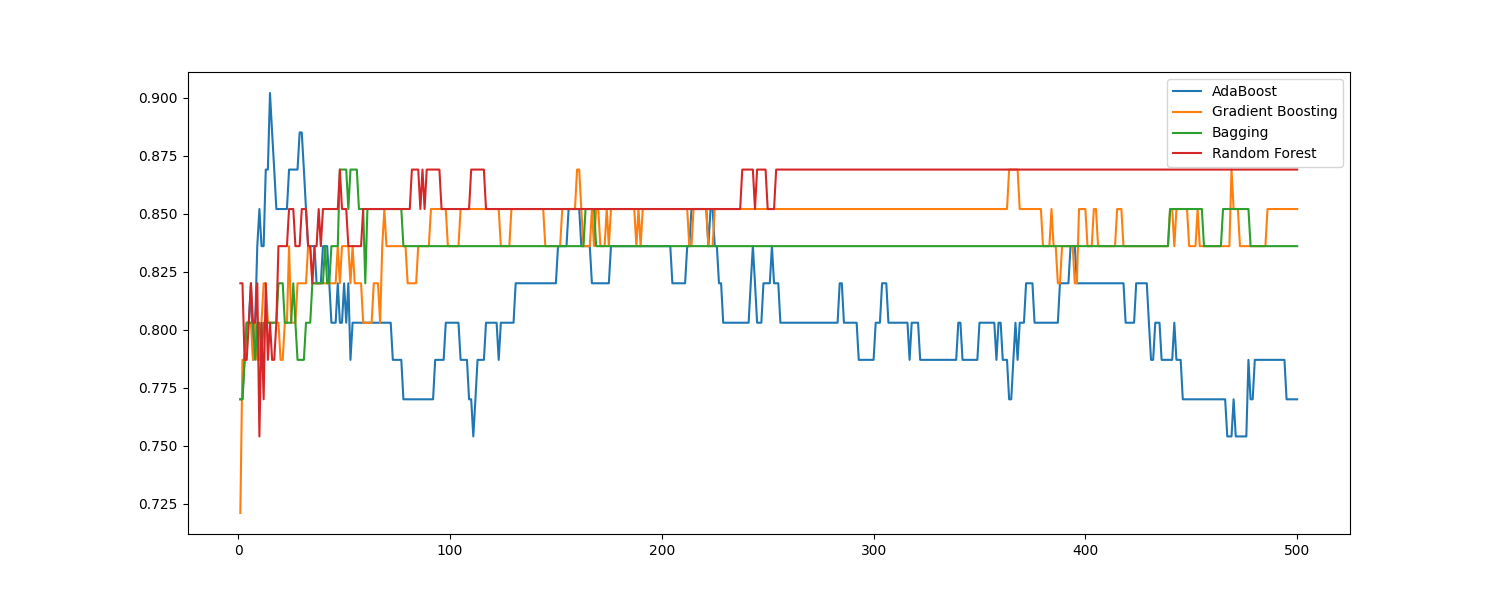
\includegraphics[width=1.23\textwidth]{figures/examples/hdc_comparison}}
    \caption{
        Accuracy comparison between the ensemble learning algorithms on the Heart Disease Cleveland dataset.
        The x-axis shows the amount of estimators and the y-axis the mean accuracy.
    }
\end{figure}

In the second example, all evaluated ensemble learning methods surpassed the decision tree in performance.
There were significant performance enhancements, ranging from 5\% up to 13\%.
Additionally, \hyperref[tab:hdc_table]{Table 2} shows that that random forest notably surpassed Bagging by
nearly 4\% in accuracy, eventhough they have the same estimator count.
Despite having the worst results on the folds, AdaBoost stood out with the highest accuracy on the validation set.
This is particularly noteworthy considering that AdaBoost utilized the fewest estimators of all methods examined,
yet managed to achieve the best performance.
The results depicted in \hyperref[fig:hdc_comparison]{Figure 7} reveal a more volatile relationship between
performance and estimator count compared to the first example. Consistent with the previous findings, the most
substantial performance improvements occurred within the initial 50 estimators.
A notable point of interest is the declining accuracy of AdaBoost as the number of estimators increase, suggesting
a tendency for the model to overfit the training data.
This underscores that more estimators can also have a negative effect on the generalizability of the model. 

\newpage % TODO: remove
\subsection{Example 3}
\label{sec:example3}

In the third example we are using the day version of the Bike Sharing dataset by
\citet*{bike_sharing}. It contains 13 features and has 731 data 
points. The goal of the dataset is to determine the amount of bikes that are going
to be rented out on the given day (regression).

\begin{table}[htbp]
    \centering
    \begin{tabular}{l c c c c c}
    \toprule
    Criteria        & DT    & Bag       & RF    & Ada   & GB \\
    \midrule
    Worst fold      & 0.606 & 0.680     & 0.680 & 0.682 & 0.749\\
    Best fold       & 0.906 & 0.925     & 0.925 & 0.943 & 0.945\\
    Average fold    & 0.771 & 0.837     & 0.838 & 0.842 & 0.868\\
    Validation      & 0.808 & 0.878     & 0.881 & 0.875 & 0.882\\
    Training time   & 0.1s  & 0.6s      & 0.5s  & 8.3s  & 0.7s\\
    Estimator count & -     & 30        & 30    & 498   & 38\\
    \bottomrule
    \end{tabular}
    \caption{
        Coefficient of determination $R^2$ on the Bike Sharing dataset using 
        (1) a decision tree (DT) regressor;
        (2) a Bagging (Bag) regressor;
        (3) a Random forest (RF) regressor; 
        (4) a AdaBoost (Ada) regressor; 
        (5) a Gradient boosting (GB) regressor.
        All ensembles use a decision tree with maximum depth of five as 
        the base learning algorithm.
    }
\end{table}

\begin{figure}[htbp]
    \centering
    \label{fig:bs_comparison}
    \makebox[\textwidth]{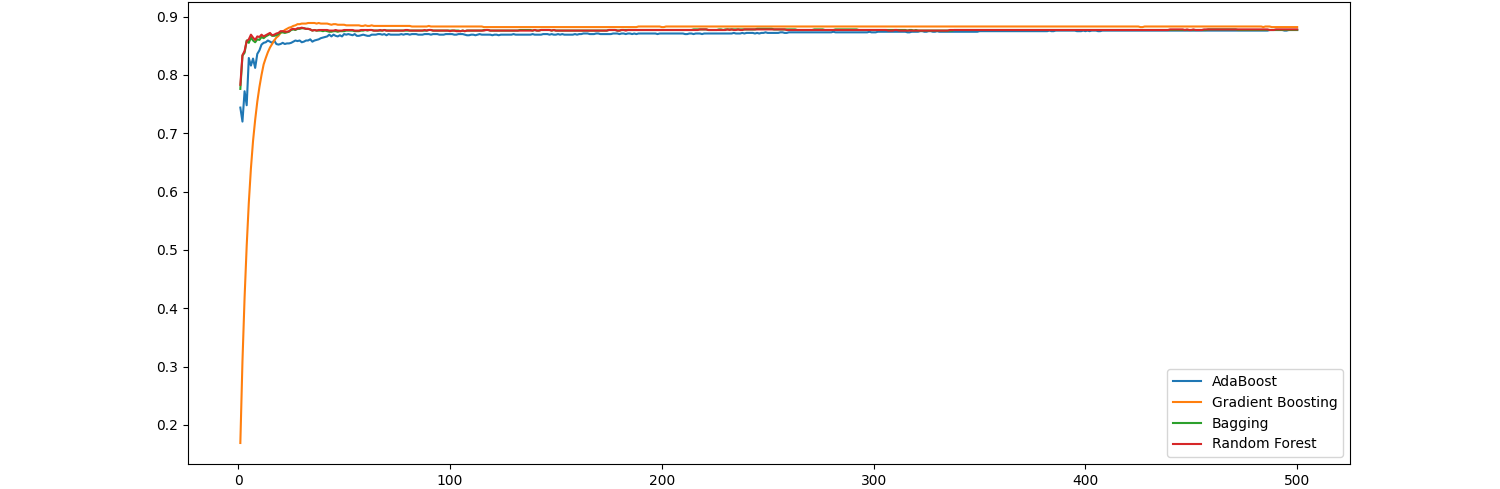
\includegraphics[width=1.23\textwidth]{figures/examples/bs_comparison}}
    \caption{
        Accuracy comparison between the ensemble learning algorithms on the Bike Sharing dataset.
        The x-axis shows the amount of estimators and the y-axis the coefficient of determination $R^2$.
    }
\end{figure}

In the third example, all ensemble methods evaluated surpassed the decision tree, each achieving roughly an 8\% improvement in accuracy.
The performance of the ensemble learning methods were closely matched, with a maximum variation of 0.7\%.
Similar to the previous results, Bagging and Random forest shared an identical number of estimators. However, this time the 
accuracy is very similar, with Random forest having a slightly higher accuracy.
In contrast to the previous examples, AdaBoost ranked lowest in terms of performance. Notably, it displayed a persistent
improvement, achieving its peak accuracy with 498 estimators. This suggests a potential for further incremental gains if allowed
additional computational resources.
Gradient Boosting, outperformed all other ensemble learning methods with a 0.1\% higher accuracy on the validation set than Random
Forest.
\hyperref[fig:bs_comparison]{Figure 8} reinforces a consistent observation: the majority of performance improvements are realized
within the initial 50 estimators, beyond which there is a general tendency to plateau.
However, AdaBoost stands as the exception to this rule, defying the common trend of stagnation observed in other methods.


\subsection{Discussion}
In \hyperref[sec:example3]{example 3}, Gradient Boosting emerged had the highest accuracy, while in \hyperref[sec:example2]{example 2},
AdaBoost did best. In \hyperref[sec:example1]{example 1}, both AdaBoost and Gradient Boosting surpassed the performance of Decision Tree,
Bagging, and Random Forest. 
That might indicate that at least one Boosting method, AdaBoost or Gradient Boosting, is always more accurate than the other methods.
However, research \citep{popular_ensemble_methods, comparison_ensemble_learning} indicates that there is no clear winner between these
methods. The effectiveness of each method highly depends on the characteristics of the data. Nevertheless, there are heuristics that can
guide the selection of the appropriate ensemble learning method and its hyperparameters.

Bagging and Random Forest are generally reliable methods, provided the necessary computational resources are available. These methods
also consistently outperform the Decision Tree.
AdaBoost and Gradient Boosting are able to be considerably more accurate than Bagging and Random Forest, as demonstrated in the examples.
Nonetheless, when the data is very noisy, Boosting is prone to overfitting, and might even perform worse than a Decision Tree.
This can also be seen in \hyperref[fig:bs_comparison]{Figure 7}, where accuracy of AdaBoost decreases with an increasing number of estimators.

Furthermore, the examples, as well as the studies show that the largest increase in accuracy is achieved with the first few estimators added to the 
ensemble. However, Boosting algorithms are sometimes able to improve with larger ensemble sizes. This can be seen \hyperref[fig:bs_comparison]{Figure 8}.

In conclusion, Bagging and Random Forest can be used for most problems, but Boosting methods might even be more accurate on suitable datasets. 

% ---------------------------------------------------------------------------- %
\section{Summary and conclusion}
Ensemble Learning is a powerful approach in machine learning that combines 
multiple models to produce a superior output compared to individual models.
Within ensemble learning, two primary techniques are Bagging and Boosting, 
each with its unique methodology and advantages.


Bagging aims to reduce variance in predictions. In bagging, models are trained 
independently in parallel, using different subsets of the training data.
The final prediction is typically made by aggregating the outputs of all models,
using methods like majority voting (classification) or averaging (regression).


Boosting focuses on reducing bias. In this technique, models are trained sequentially,
where each model attempts to correct the errors made by the previous one. Despite 
the sequential training, predictions can be made in parallel. Furthermore, the
performance of each model in the training step determines how strong the influence
is on the final prediction. Therefire weighted averaging is used to build a final
prediciton.


The evolution of these methods into more advanced versions like Random Forests
and Gradient Boosting has further enhanced their capabilities. These advanced 
techniques can outperform standard individual models and even the basic forms 
of bagging and boosting. 


The choice between the model should be guided by the specific requirements of 
the problem at hand, considering factors like data characteristics, computing 
resources, and the inherent trade-offs between bias and variance.
